% Options for packages loaded elsewhere
\PassOptionsToPackage{unicode}{hyperref}
\PassOptionsToPackage{hyphens}{url}
%
\documentclass[
  11pt,
  ignorenonframetext,
  aspectratio=169,
  c]{beamer}
\usepackage{pgfpages}
\setbeamertemplate{caption}[numbered]
\setbeamertemplate{caption label separator}{: }
\setbeamercolor{caption name}{fg=normal text.fg}
\beamertemplatenavigationsymbolshorizontal
% Prevent slide breaks in the middle of a paragraph
\widowpenalties 1 10000
\raggedbottom
\setbeamertemplate{part page}{
  \centering
  \begin{beamercolorbox}[sep=16pt,center]{part title}
    \usebeamerfont{part title}\insertpart\par
  \end{beamercolorbox}
}
\setbeamertemplate{section page}{
  \centering
  \begin{beamercolorbox}[sep=12pt,center]{part title}
    \usebeamerfont{section title}\insertsection\par
  \end{beamercolorbox}
}
\setbeamertemplate{subsection page}{
  \centering
  \begin{beamercolorbox}[sep=8pt,center]{part title}
    \usebeamerfont{subsection title}\insertsubsection\par
  \end{beamercolorbox}
}
\AtBeginPart{
  \frame{\partpage}
}
\AtBeginSection{
  \ifbibliography
  \else
    \frame{\sectionpage}
  \fi
}
\AtBeginSubsection{
  \frame{\subsectionpage}
}

\usepackage{amsmath,amssymb}
\usepackage{lmodern}
\usepackage{iftex}
\ifPDFTeX
  \usepackage[T1]{fontenc}
  \usepackage[utf8]{inputenc}
  \usepackage{textcomp} % provide euro and other symbols
\else % if luatex or xetex
  \usepackage{unicode-math}
  \defaultfontfeatures{Scale=MatchLowercase}
  \defaultfontfeatures[\rmfamily]{Ligatures=TeX,Scale=1}
\fi
\usetheme[]{Luebeck}
\usecolortheme{beaver}
% Use upquote if available, for straight quotes in verbatim environments
\IfFileExists{upquote.sty}{\usepackage{upquote}}{}
\IfFileExists{microtype.sty}{% use microtype if available
  \usepackage[]{microtype}
  \UseMicrotypeSet[protrusion]{basicmath} % disable protrusion for tt fonts
}{}
\makeatletter
\@ifundefined{KOMAClassName}{% if non-KOMA class
  \IfFileExists{parskip.sty}{%
    \usepackage{parskip}
  }{% else
    \setlength{\parindent}{0pt}
    \setlength{\parskip}{6pt plus 2pt minus 1pt}}
}{% if KOMA class
  \KOMAoptions{parskip=half}}
\makeatother
\usepackage{xcolor}
\newif\ifbibliography
\setlength{\emergencystretch}{3em} % prevent overfull lines
\setcounter{secnumdepth}{-\maxdimen} % remove section numbering


\providecommand{\tightlist}{%
  \setlength{\itemsep}{0pt}\setlength{\parskip}{0pt}}\usepackage{longtable,booktabs,array}
\usepackage{calc} % for calculating minipage widths
\usepackage{caption}
% Make caption package work with longtable
\makeatletter
\def\fnum@table{\tablename~\thetable}
\makeatother
\usepackage{graphicx}
\makeatletter
\def\maxwidth{\ifdim\Gin@nat@width>\linewidth\linewidth\else\Gin@nat@width\fi}
\def\maxheight{\ifdim\Gin@nat@height>\textheight\textheight\else\Gin@nat@height\fi}
\makeatother
% Scale images if necessary, so that they will not overflow the page
% margins by default, and it is still possible to overwrite the defaults
% using explicit options in \includegraphics[width, height, ...]{}
\setkeys{Gin}{width=\maxwidth,height=\maxheight,keepaspectratio}
% Set default figure placement to htbp
\makeatletter
\def\fps@figure{htbp}
\makeatother

\usepackage{tabu}

%\usepackage{emoji}
%\usepackage{xelatexemoji}-
%\AtBeginSection{}
%\renewcommand{\tableofcontents}{...}
%\setbeameroption{show notes}
%\setbeamertemplate{navigation symbols}{}
%\setbeamertemplate{footline}[page number]
        
\usepackage{appendixnumberbeamer}
\makeatletter
\makeatother
\makeatletter
\makeatother
\makeatletter
\@ifpackageloaded{caption}{}{\usepackage{caption}}
\AtBeginDocument{%
\ifdefined\contentsname
  \renewcommand*\contentsname{Table of contents}
\else
  \newcommand\contentsname{Table of contents}
\fi
\ifdefined\listfigurename
  \renewcommand*\listfigurename{List of Figures}
\else
  \newcommand\listfigurename{List of Figures}
\fi
\ifdefined\listtablename
  \renewcommand*\listtablename{List of Tables}
\else
  \newcommand\listtablename{List of Tables}
\fi
\ifdefined\figurename
  \renewcommand*\figurename{Figure}
\else
  \newcommand\figurename{Figure}
\fi
\ifdefined\tablename
  \renewcommand*\tablename{Table}
\else
  \newcommand\tablename{Table}
\fi
}
\@ifpackageloaded{float}{}{\usepackage{float}}
\floatstyle{ruled}
\@ifundefined{c@chapter}{\newfloat{codelisting}{h}{lop}}{\newfloat{codelisting}{h}{lop}[chapter]}
\floatname{codelisting}{Listing}
\newcommand*\listoflistings{\listof{codelisting}{List of Listings}}
\makeatother
\makeatletter
\@ifpackageloaded{caption}{}{\usepackage{caption}}
\@ifpackageloaded{subcaption}{}{\usepackage{subcaption}}
\makeatother
\makeatletter
\@ifpackageloaded{tcolorbox}{}{\usepackage[many]{tcolorbox}}
\makeatother
\makeatletter
\@ifundefined{shadecolor}{\definecolor{shadecolor}{rgb}{.97, .97, .97}}
\makeatother
\makeatletter
\makeatother
\ifLuaTeX
  \usepackage{selnolig}  % disable illegal ligatures
\fi
\IfFileExists{bookmark.sty}{\usepackage{bookmark}}{\usepackage{hyperref}}
\IfFileExists{xurl.sty}{\usepackage{xurl}}{} % add URL line breaks if available
\urlstyle{same} % disable monospaced font for URLs
\hypersetup{
  pdftitle={Candidature au poste de   Maître de Conférences},
  pdfauthor={Fabio A. CRUZ SANCHEZ   Section CNU 60},
  hidelinks,
  pdfcreator={LaTeX via pandoc}}

\title{Candidature au poste de Maître de Conférences}
\subtitle{ENSGSI / ERPI}
\author{Fabio A. CRUZ SANCHEZ Section CNU 60}
\date{Invalid Date}

\begin{document}
\frame{\titlepage}
\ifdefined\Shaded\renewenvironment{Shaded}{\begin{tcolorbox}[boxrule=0pt, breakable, interior hidden, borderline west={3pt}{0pt}{shadecolor}, enhanced, sharp corners, frame hidden]}{\end{tcolorbox}}\fi

\begin{frame}
\section*{Appendix}

\appendix
\end{frame}

\begin{frame}[t]{Domaine de recherche}
\protect\hypertarget{domaine-de-recherche}{}
\emph{Recyclage distribué} via open source hardware: Validation
multi-echelle.

\begin{enumerate}
\tightlist
\item
  Feasabilité technique
\item
  Filière en circuit court
\item
  (E)valuation sur le territoire
\end{enumerate}

\begin{tikzpicture}[remember picture,overlay]
    \node[xshift=1.5cm,yshift=-1.3cm] at (current page.center) {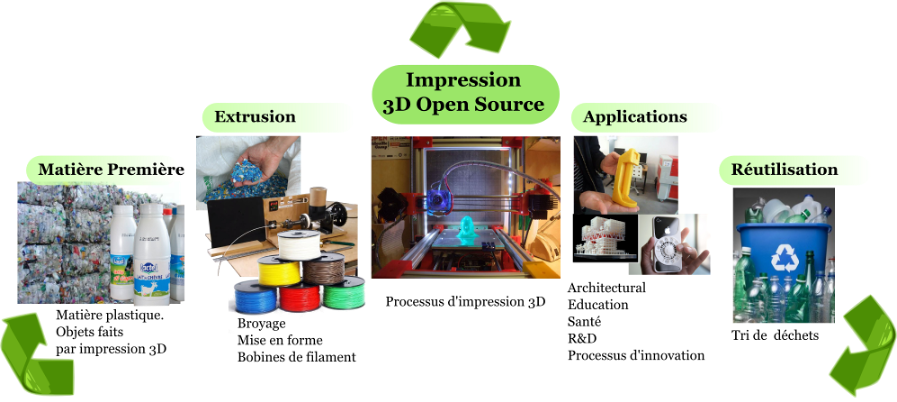
\includegraphics[width=12cm]{Figures/slides/DRAM-00.png}};
\end{tikzpicture}
\end{frame}

\begin{frame}[t]{Domaine de recherche}
\protect\hypertarget{domaine-de-recherche-1}{}
\emph{Recyclage distribué} via fabrication additive open source:
Validation multi-echelle.

\begin{columns}[T]
\begin{column}[T]{0.65\textwidth}
\small

\begin{enumerate}
\tightlist
\item
  Feasabilité technique la fabrication additive open source
\item
  Filière en boucle (semi) fermé et en circuit court
\item
  (E)valuation sur le territoire
\end{enumerate}

\begin{figure}

{\centering 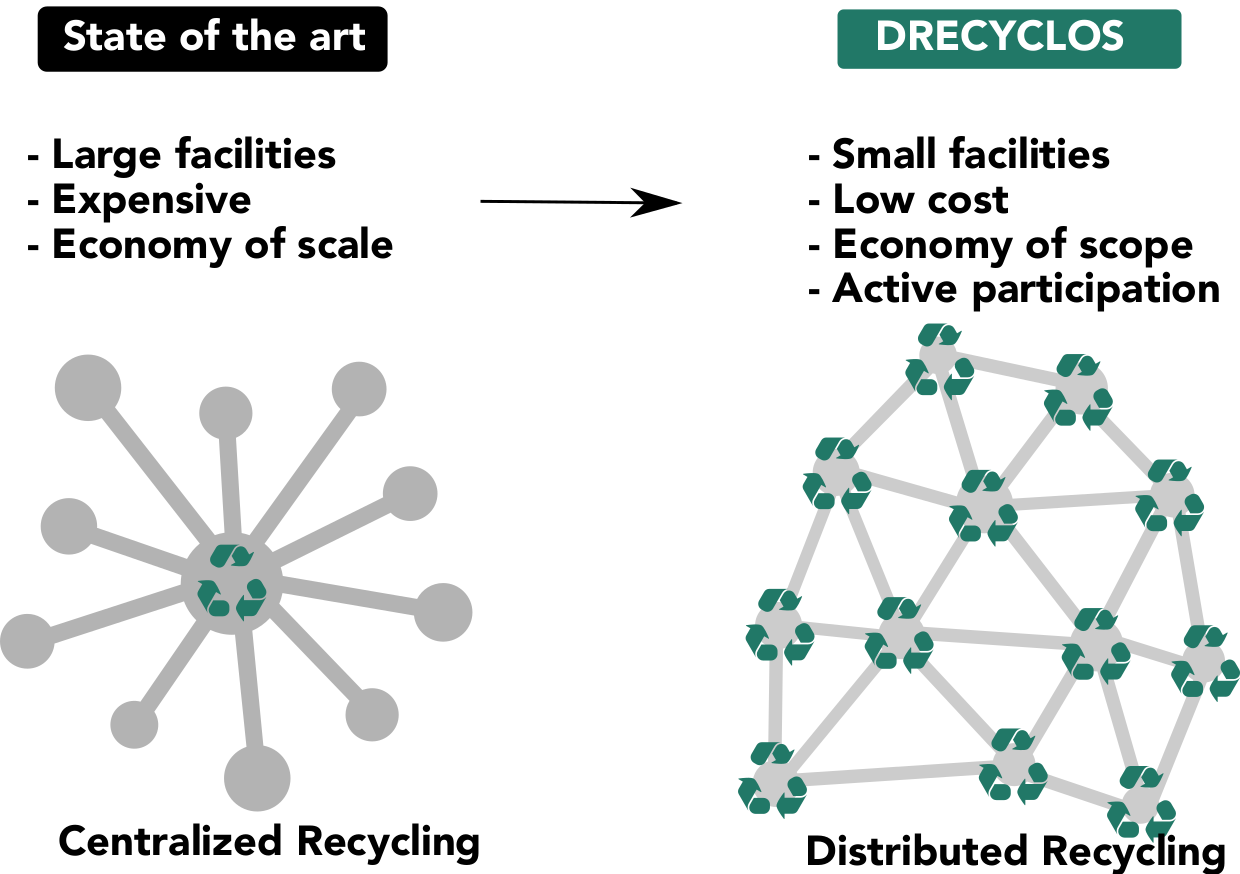
\includegraphics[width=1.5625in,height=\textheight]{Figures/slides/Abstract.png}

}

\end{figure}
\end{column}

\begin{column}[T]{0.35\textwidth}
\begin{figure}

{\centering 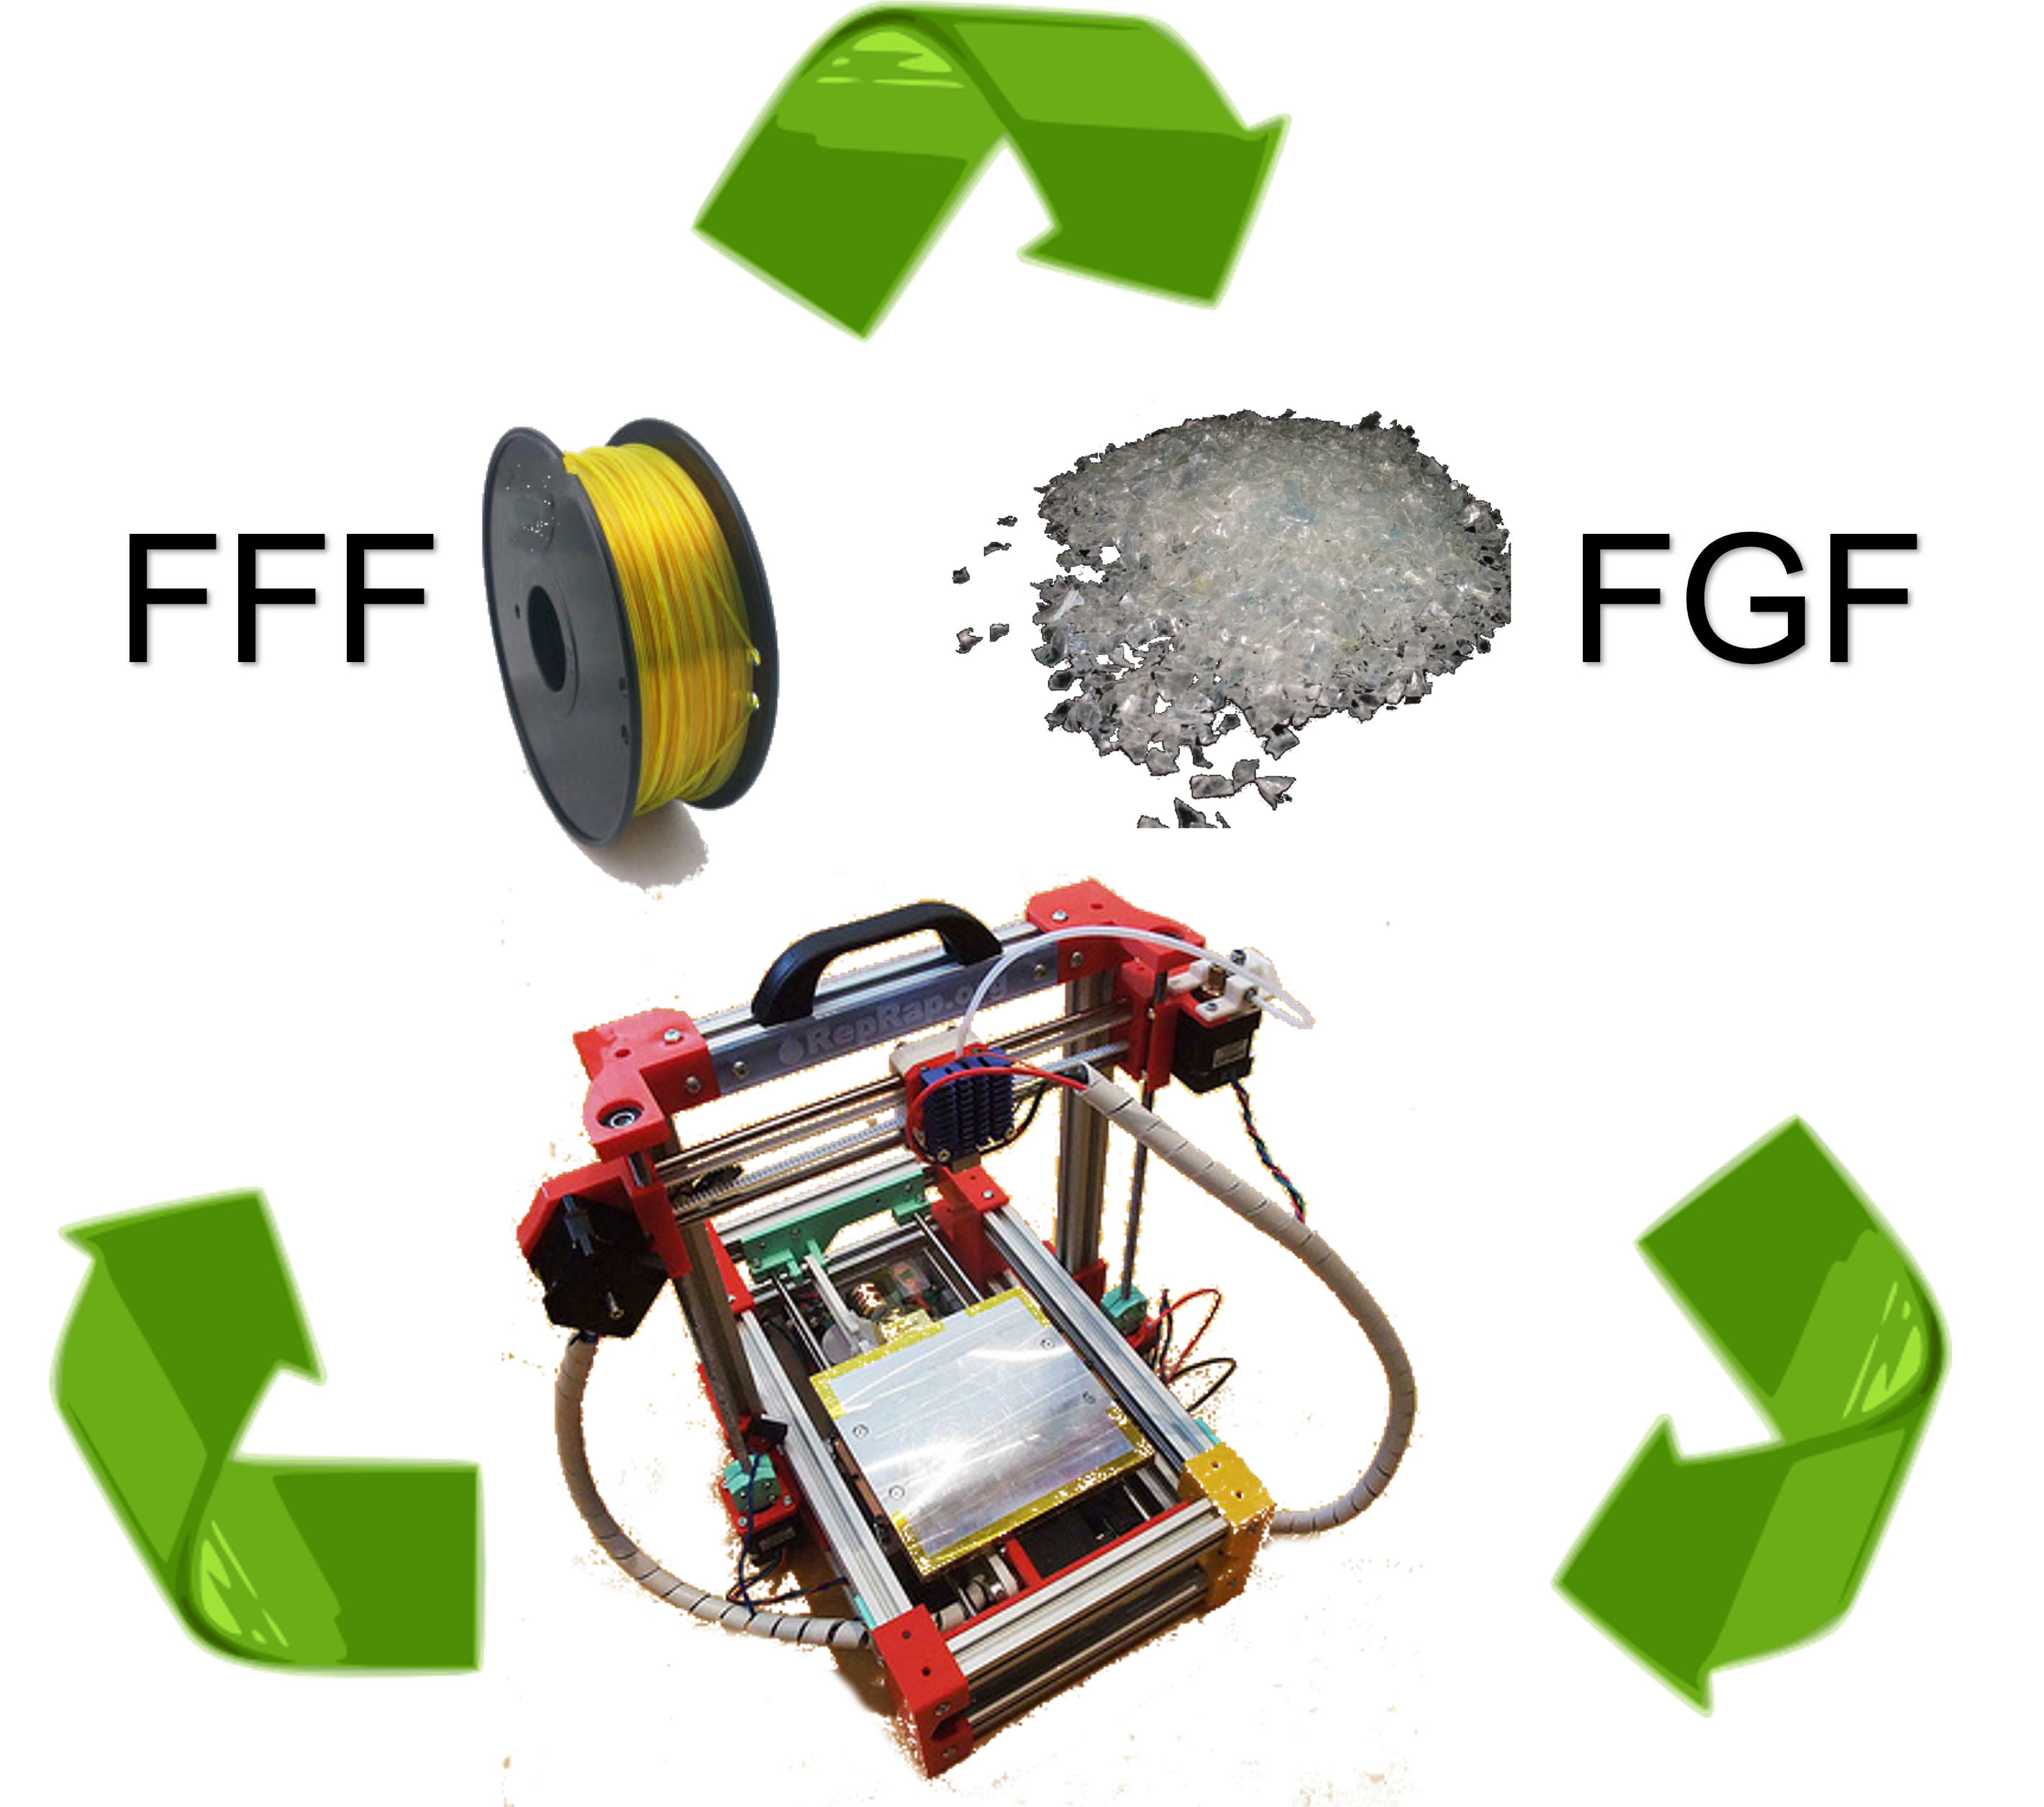
\includegraphics[width=2.08333in,height=\textheight]{Figures/slides/Recherche-Intro-01.png}

}

\end{figure}
\end{column}
\end{columns}
\end{frame}

\begin{frame}[t]{Echelles de Recherche}
\protect\hypertarget{echelles-de-recherche}{}
\emph{Recyclage distribué} via open source hardware: \textbf{Validation
multi-echelle}

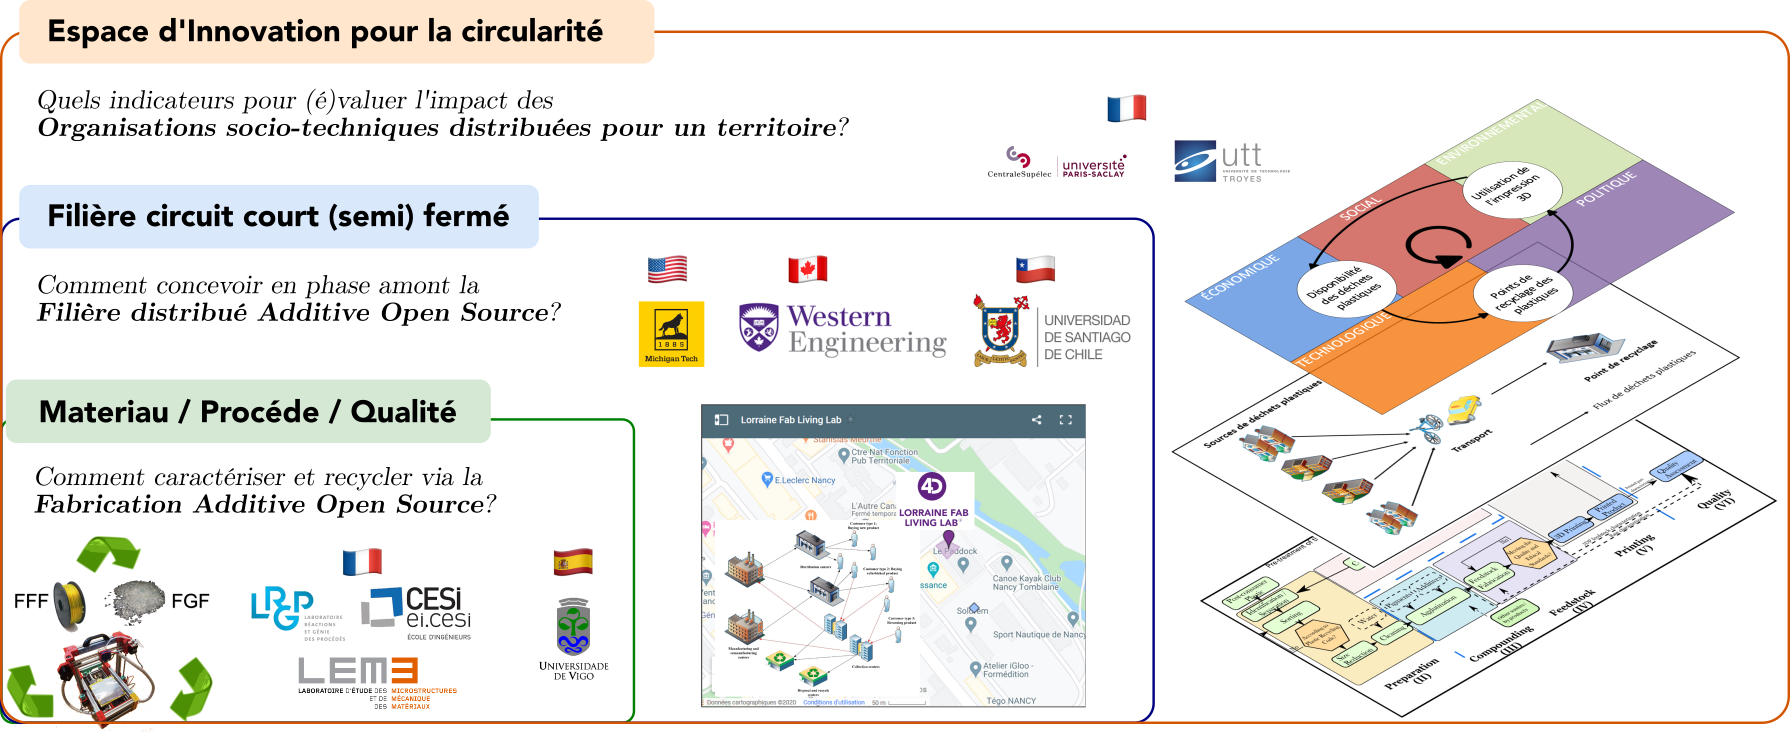
\includegraphics[width=0.9\textwidth,height=\textheight]{Figures/slides/recherche-fabio.png}

\note{}
\end{frame}

\begin{frame}[t]{Module CI15 - Recherche, Developpement et Innovation}
\protect\hypertarget{module-ci15---recherche-developpement-et-innovation}{}
\begin{columns}[T]
\begin{column}[c]{0.5\textwidth}
\scriptsize

\textbf{Objectif:}

\begin{itemize}
\tightlist
\item
  Recherche an tant que compétence transversal.
\item
  Lien entre la \textbf{recherche et leur sujet de stage!}.
\item
  Devenir un interlocuteur valable via la recherche.
\end{itemize}
\end{column}

\begin{column}[c]{0.5\textwidth}
\scriptsize

\begin{itemize}
\tightlist
\item
  Niveau BAC+5: ENSGSI 3AI, Master M2 IDEAS \& IUVTT
\end{itemize}
\end{column}
\end{columns}

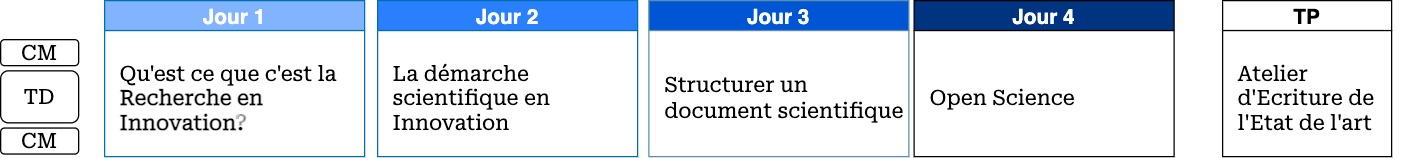
\includegraphics{figures/slides/Ensegnement-CI15.jpg}
\end{frame}

\hypertarget{projet-de-recherche}{%
\subsection{Projet de Recherche}\label{projet-de-recherche}}

\begin{frame}{Projet de Recherche}
Green Fablab comme projet federateur et transversal pour ERPI:

\begin{columns}[T]
\begin{column}[T]{0.3\textwidth}
\footnotesize

\begin{itemize}
\item
  Nouveaux démonstrateurs et protocoles expérimentaux Open Source
\item
  Recherche fondamental vers Recherche-action
\item
  (E)valuation Multi-acteurs et Multi-echelle
\end{itemize}
\end{column}

\begin{column}[T]{0.7\textwidth}
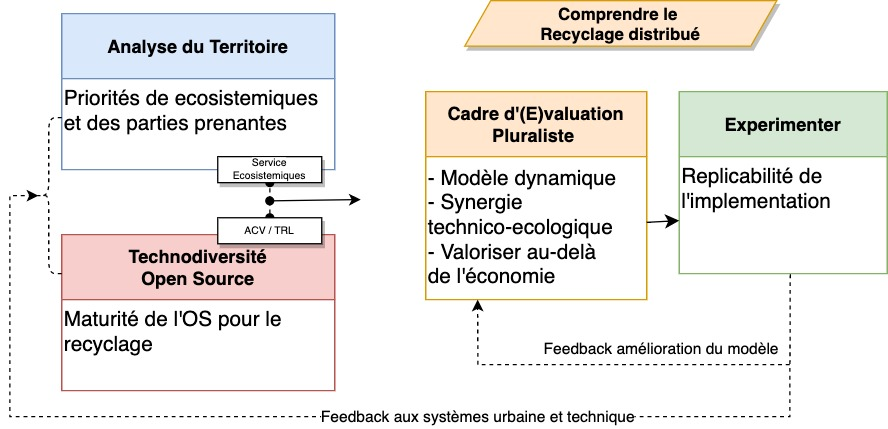
\includegraphics{Figures/slides/Projet-Recherche.jpg}
\end{column}
\end{columns}
\end{frame}

\begin{frame}[t]{Génie Mécanique et Energetique}
\protect\hypertarget{guxe9nie-muxe9canique-et-energetique}{}
Caractérisation des matériaux en utilisant l'approche open hardware
comme support pédagogique

\begin{block}{Travail sur un cas d'étude :}
\protect\hypertarget{travail-sur-un-cas-duxe9tude}{}
Conception, fabrication et simulation d'un ailette thermique open
source?
\end{block}
\end{frame}

\begin{frame}{(Re)conception et Innovation en mode Green Fablab}
\protect\hypertarget{reconception-et-innovation-en-mode-green-fablab}{}
La (\emph{Re})conception de produit en utilisant des critères de
soutenabilité.

\begin{block}{Travail sur un cas d'étude :}
\protect\hypertarget{travail-sur-un-cas-duxe9tude-1}{}
\end{block}
\end{frame}

\begin{frame}{3AI: Parcours}
\protect\hypertarget{ai-parcours}{}
Open design pour la soutenabilité: les atouts de la collecte jusqu'au
recyclage en circuit court
\end{frame}

\hypertarget{quarto}{%
\subsection{Quarto}\label{quarto}}

\begin{frame}{Quarto}
Quarto enables you to weave together content and executable code into a
finished document. To learn more about Quarto see
\url{https://quarto.org}.
\end{frame}

\hypertarget{running-code}{%
\subsection{Running Code}\label{running-code}}

\begin{frame}[fragile]{Running Code}
When you click the \textbf{Render} button a document will be generated
that includes both content and the output of embedded code. You can
embed code like this:

\begin{verbatim}
[1] 2
\end{verbatim}

You can add options to executable code like this

\begin{verbatim}
[1] 4
\end{verbatim}

The \texttt{echo:\ false} option disables the printing of code (only
output is displayed).
\end{frame}



\end{document}
